% Provenance (never printed): 6e geography and cycle 3 sciences (locating a
% place on the globe: parallels, meridians, latitude, longitude; the Earth's
% rotation and time zones); see sources/book1/PROVENANCE.md.
% Book 1, grade 6, chapter 2.
\chapter{Lintang, Bujur, dan Zona Waktu}\label{ch:g6:latitude-longitude}

Malam telah turun di \omterm{def:g2:water-on-earth:ocean}{samudra}. Di geladak sebuah kapal layar, pada tahun
1750, sang navigator mengangkat alatnya ke arah sebuah bintang yang terang
dan mengukur seberapa tinggi bintang itu di atas \omterm{def:g2:water-on-earth:ocean}{laut}. Beberapa menit
bekerja, dan ia tahu seberapa jauh kapal itu berada di utara \omterm{def:g3:continents-and-oceans:equator}{khatulistiwa}.
Akan tetapi, seberapa jauh ke timur atau ke barat? Hal itu tidak dapat
diketahuinya. Masalah ini begitu serius sehingga pada tahun 1714 parlemen
Inggris menjanjikan hadiah besar bagi siapa saja yang menemukan cara untuk
mengukurnya di \omterm{def:g2:water-on-earth:ocean}{laut}. Sekarang, ponsel di sakumu memberikan kedua jawaban itu
dalam satu detik.
% ledger: rmg:15deg-per-hour, rmg:longitude-act-1714

\begin{omfigure}
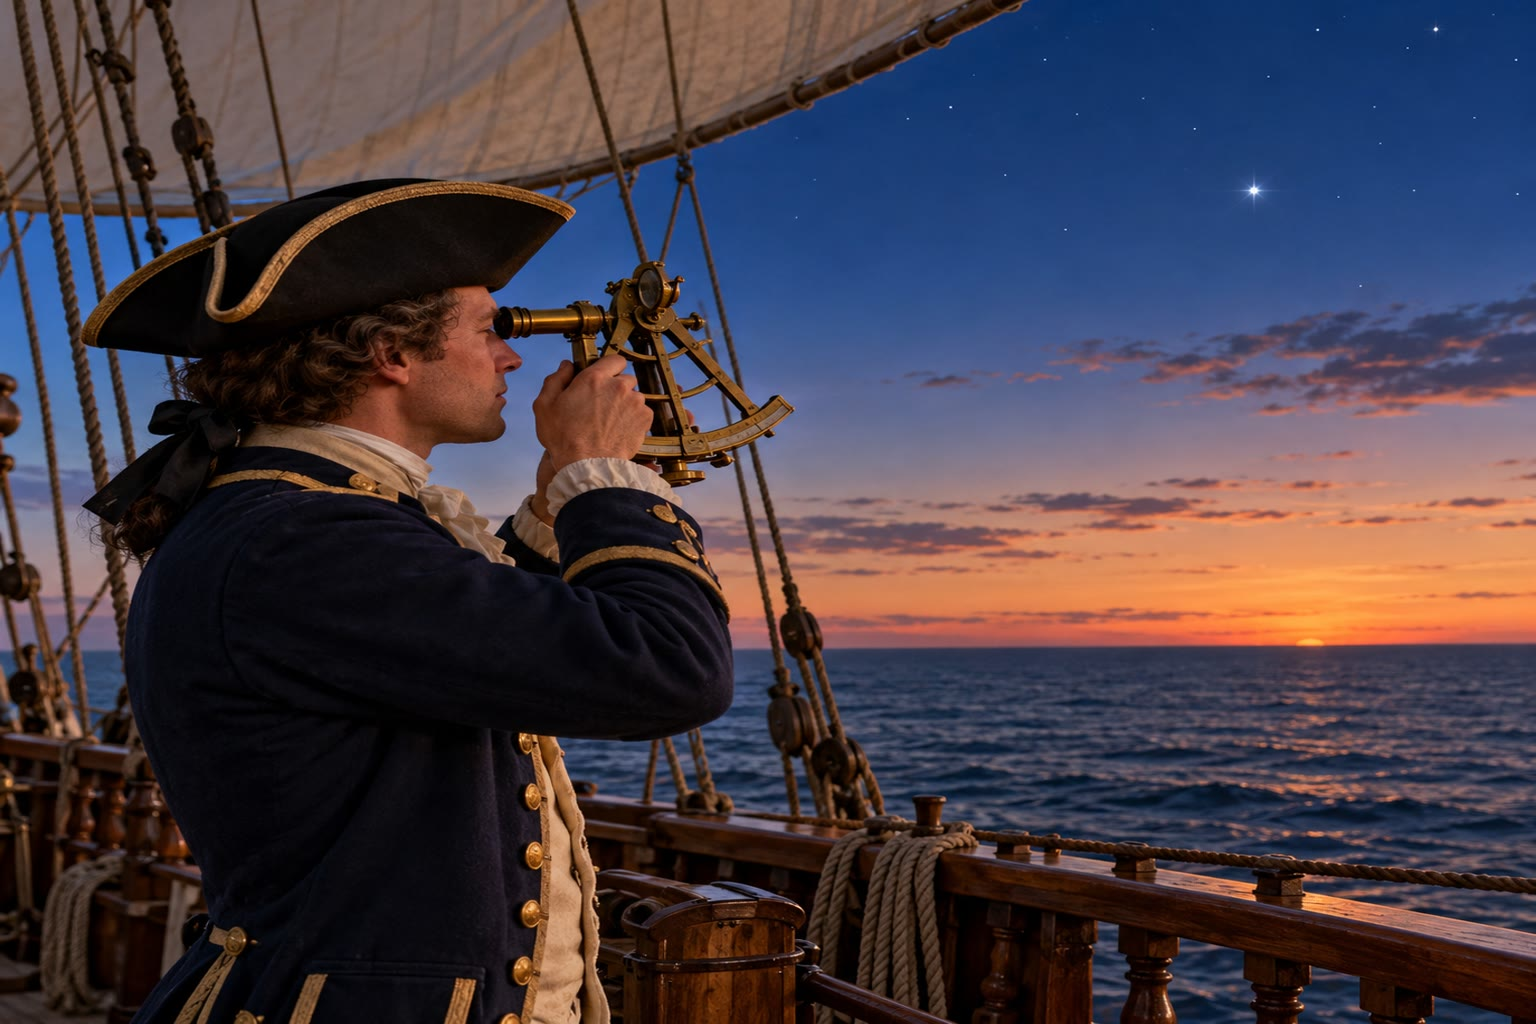
\includegraphics[width=0.62\linewidth]{images/book1/ai/g6-navigator-sextant.jpg}

{\small Seorang navigator abad kedelapan belas mengukur tinggi sebuah bintang
di atas cakrawala \omterm{def:g2:water-on-earth:ocean}{laut}. (Ilustrasi AI.)}
\end{omfigure}

\begin{recall}
\omterm{def:g3:continents-and-oceans:globe}{Bola dunia} adalah model kecil Bumi. \omterm{def:g3:continents-and-oceans:equator}{Khatulistiwa} adalah garis yang
melingkari bagian tengah \omterm{def:g3:continents-and-oceans:globe}{bola dunia}, di pertengahan antara \omterm{def:g3:continents-and-oceans:poles}{Kutub Utara} dan
\omterm{def:g3:continents-and-oceans:poles}{Kutub Selatan}; garis itu membelah Bumi menjadi \omterm{def:g3:continents-and-oceans:equator}{belahan bumi utara} dan
\omterm{def:g3:continents-and-oceans:equator}{belahan bumi selatan} (\cref{ch:g3:continents-and-oceans}). Buku fisika telah
menunjukkan bahwa Bumi berputar pada dirinya sendiri di sekitar sumbu yang
melalui kedua \omterm{def:g3:continents-and-oceans:poles}{kutub}, satu kali dalam sehari: perputaran inilah yang
menyebabkan siang dan malam.
\end{recall}

\section{Paralel dan lintang}

Untuk menyatakan letak suatu tempat di Bumi, kita memerlukan dua angka,
seperti baris dan kolom sebuah kursi di bioskop. Angka pertama menunjukkan
seberapa jauh di utara atau di selatan \omterm{def:g3:continents-and-oceans:equator}{khatulistiwa} tempat itu terletak.

Bayangkan Bumi dibelah dua, melalui kedua \omterm{def:g3:continents-and-oceans:poles}{kutub}, seperti apel yang dibelah
dari tangkainya ke bawah. Pada bidang belahannya (kiri, di bawah),
\omterm{def:g3:continents-and-oceans:equator}{khatulistiwa} adalah garis mendatar yang melalui pusat. Sebuah tempat~P di
permukaan terlihat dari pusat pada sudut tertentu di atas atau di bawah
garis itu: sudut inilah \omterm{def:g6:latitude-longitude:latitude}{lintangnya}.

\begin{omfigure}
\begin{minipage}[t]{0.48\linewidth}\centering
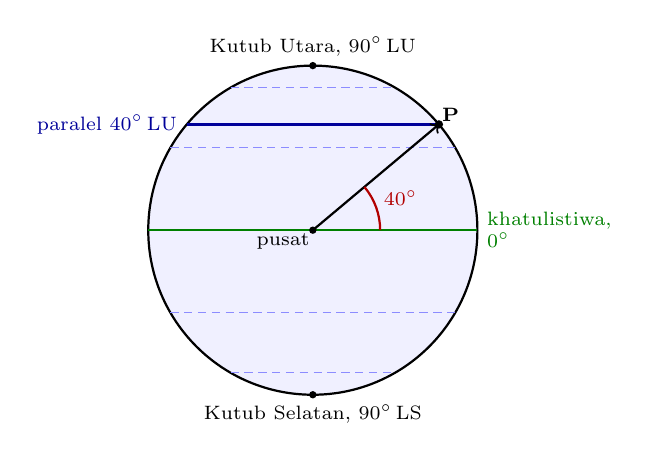
\begin{tikzpicture}[scale=0.95]
  \def\R{2.2}
  \fill[blue!6] (0,0) circle (\R);
  \draw[thick] (0,0) circle (\R);
  % parallels seen edge-on: horizontal chords
  \foreach \a in {-60,-30,30,60}{
    \draw[blue!45, densely dashed] ({-\R*cos(\a)},{\R*sin(\a)}) -- ({\R*cos(\a)},{\R*sin(\a)});}
    \draw[green!50!black, thick] (-\R,0) -- (\R,0);
  \node[font=\scriptsize, green!50!black, anchor=west, align=left] at (\R,0) {khatulistiwa,\\ $0^\circ$};
  \draw[blue!60!black, thick] ({-\R*cos(40)},{\R*sin(40)}) -- ({\R*cos(40)},{\R*sin(40)});
  \draw[->, thick] (0,0) -- ({\R*cos(40)},{\R*sin(40)});
  \fill (0,0) circle (1.4pt) node[below left, font=\scriptsize, inner sep=1pt] {pusat};
  \fill ({\R*cos(40)},{\R*sin(40)}) circle (1.6pt)
    node[above right, font=\scriptsize\bfseries, inner sep=1pt] {P};
  \draw[red!70!black, thick] (0.9,0) arc (0:40:0.9);
  \node[red!70!black, font=\scriptsize] at (20:1.25) {$40^\circ$};
  \node[font=\scriptsize, blue!60!black, anchor=east] at ({-\R*cos(40)},{\R*sin(40)}) {paralel $40^\circ$\,LU};
  \fill (0,\R) circle (1.4pt) node[above, font=\scriptsize] {Kutub Utara, $90^\circ$\,LU};
  \fill (0,-\R) circle (1.4pt) node[below, font=\scriptsize] {Kutub Selatan, $90^\circ$\,LS};
\end{tikzpicture}

{\small \omterm{def:g6:latitude-longitude:latitude}{Lintang}: sudut di pusat Bumi antara \omterm{def:g3:continents-and-oceans:equator}{khatulistiwa} dan tempat itu.}
\end{minipage}\hfill
\begin{minipage}[t]{0.48\linewidth}\centering
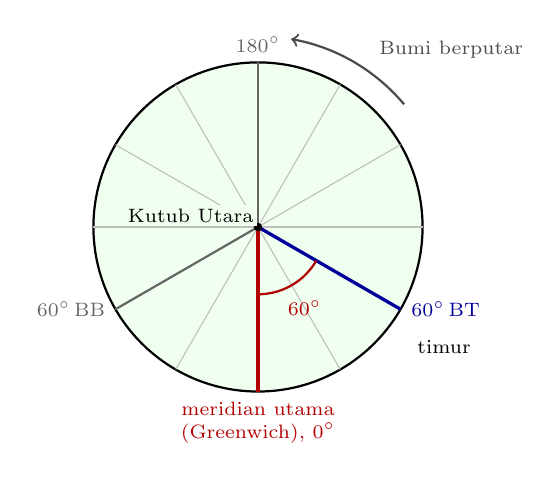
\begin{tikzpicture}[scale=0.95]
  \def\R{2.2}
  \fill[green!6] (0,0) circle (\R);
  \draw[thick] (0,0) circle (\R);
  \foreach \a in {0,30,...,330}{\draw[black!25] (0,0) -- (\a:\R);}
    \draw[red!70!black, very thick] (0,0) -- (270:\R)
    node[below, font=\scriptsize, align=center] {meridian utama\\(Greenwich), $0^\circ$};
  \draw[blue!60!black, very thick] (0,0) -- (330:\R)
    node[right, font=\scriptsize] {$60^\circ$\,BT};
  \draw[black!60, thick] (0,0) -- (210:\R) node[left, font=\scriptsize] {$60^\circ$\,BB};
  \draw[black!60, thick] (0,0) -- (90:\R) node[above, font=\scriptsize] {$180^\circ$};
  \draw[red!70!black, thick] (270:0.9) arc (270:330:0.9);
  \node[red!70!black, font=\scriptsize] at (300:1.25) {$60^\circ$};
    \fill (0,0) circle (1.6pt) node[above left, font=\scriptsize, inner sep=1.5pt, fill=green!6] {Kutub Utara};
  \draw[->, thick, black!70] (40:2.55) arc (40:80:2.55);
  \node[font=\scriptsize, black!70, anchor=south west] at (55:2.6) {Bumi berputar};
  \node[font=\scriptsize, anchor=west] at (2.0,-1.6) {timur $\circlearrowleft$};
\end{tikzpicture}

{\small \omterm{def:g6:latitude-longitude:longitude}{Bujur}: Bumi dilihat dari atas \omterm{def:g3:continents-and-oceans:poles}{Kutub Utara}. Sudutnya diukur dari
\omterm{def:g6:latitude-longitude:longitude}{meridian utama}, ke arah timur atau ke arah barat.}
\end{minipage}
% ledger: rmg:latitude-def, rmg:longitude-def
\end{omfigure}

\begin{definition}[Paralel dan lintang]\label{def:g6:latitude-longitude:latitude}
Yang disebut \emph{paralel}\index{paralel} adalah lingkaran yang digambar
mengelilingi \omterm{def:g3:continents-and-oceans:globe}{bola dunia} sejajar dengan \omterm{def:g3:continents-and-oceans:equator}{khatulistiwa}; semua tempat pada
paralel yang sama berjarak sama dari \omterm{def:g3:continents-and-oceans:equator}{khatulistiwa}. Yang disebut
\emph{lintang}\index{lintang} suatu tempat adalah sudut, yang diukur di pusat
Bumi, antara \omterm{def:g3:continents-and-oceans:equator}{khatulistiwa} dan tempat itu. Lintang bernilai dari $0^\circ$ di
\omterm{def:g3:continents-and-oceans:equator}{khatulistiwa} sampai $90^\circ$ di \omterm{def:g3:continents-and-oceans:poles}{kutub}, dan kita menyebutkan apakah tempat
itu berada di utara (lintang utara, LU) atau di selatan (lintang selatan,
LS) \omterm{def:g3:continents-and-oceans:equator}{khatulistiwa}.
% ledger: rmg:latitude-def
\end{definition}

\omterm{def:g3:continents-and-oceans:equator}{Khatulistiwa} sendiri adalah sebuah \omterm{def:g6:latitude-longitude:latitude}{paralel}, yang paling panjang, dengan
\omterm{def:g6:latitude-longitude:latitude}{lintang} $0^\circ$. \omterm{def:g6:latitude-longitude:latitude}{Paralel-paralel} makin pendek ke arah \omterm{def:g3:continents-and-oceans:poles}{kutub}, dan setiap
\omterm{def:g3:continents-and-oceans:poles}{kutub} hanyalah sebuah titik, pada $90^\circ$\,LU atau $90^\circ$\,LS. Di
sepanjang garis dari sebuah \omterm{def:g3:continents-and-oceans:poles}{kutub} ke \omterm{def:g3:continents-and-oceans:equator}{khatulistiwa}, setiap derajat \omterm{def:g6:latitude-longitude:latitude}{lintang}
panjangnya kira-kira \qty{111}{km}.
% ledger: rmg:latitude-def

\omterm{def:g6:latitude-longitude:latitude}{Lintang} adalah angka yang mudah: \omterm{def:g6:latitude-longitude:latitude}{lintang} dapat ditentukan dari langit. Pada
siang hari, para pelaut mengukur tinggi Matahari pada tengah hari; pada
malam hari, di \omterm{def:g3:continents-and-oceans:equator}{belahan bumi utara}, mereka mengukur tinggi Bintang Utara.
Itulah yang sedang dilakukan navigator pada gambar pembuka.
% ledger: rmg:15deg-per-hour

Bintang Utara terletak hampir tepat pada garis sumbu Bumi yang
diperpanjang melewati \omterm{def:g3:continents-and-oceans:poles}{Kutub Utara}, dan begitu jauh sehingga cahayanya
mencapai setiap tempat di Bumi sepanjang garis-garis yang sejajar. Di \omterm{def:g3:continents-and-oceans:poles}{Kutub
Utara}, bintang itu tepat di atas kepala, pada $90^\circ$ di atas cakrawala;
di \omterm{def:g3:continents-and-oceans:equator}{khatulistiwa}, bintang itu terletak di cakrawala utara, pada $0^\circ$. Di
antara keduanya, aturannya sederhana: \emph{tinggi Bintang Utara di atas
cakrawala utara, yang diukur sebagai sudut, sama dengan \omterm{def:g6:latitude-longitude:latitude}{lintang}}. Gambar di
bawah ini menunjukkan mengapa kedua sudut itu sama.
% ledger: nsta:polaris-latitude

\begin{omfigure}
\begin{tikzpicture}[scale=1.1, font=\scriptsize]
  \def\R{1.7}
  \coordinate (O) at (0,0);
  \coordinate (P) at ({\R*cos(40)},{\R*sin(40)});
  \fill[blue!8] (O) circle (\R);
  \draw[black!70] (O) circle (\R);
  % equator and axis
  \draw[black!50] (-\R,0) -- (\R,0);
  \node[black!60, anchor=north east] at (-0.15,0) {khatulistiwa};
  \draw[black!70, -{Stealth[length=2mm]}] (0,-\R-0.3) -- (0,\R+1.7);
  \node[anchor=east, align=right] at (-0.1,\R+1.45) {ke arah Bintang Utara\\(sangat jauh)};
  \node[anchor=south east] at (0,\R) {U};
  % radius to P and latitude angle at the centre
  \draw[black!80] (O) -- (P);
  \draw[red!70!black, thick] (0.55,0) arc (0:40:0.55);
  \node[red!70!black] at (20:0.8) {$40^\circ$};
  % horizon at P (tangent) and the ray to the Pole Star (parallel to the axis)
  \draw[black!70, thick] ($(P)+({-sin(40)*1.5},{cos(40)*1.5})$) -- ($(P)+({sin(40)*1.6},{-cos(40)*1.6})$);
  \node[anchor=south, rotate=-50, inner sep=2pt] at ($(P)+({sin(40)*1.15},{-cos(40)*1.15})$) {cakrawala};
  \draw[orange!80!black, thick, -{Stealth[length=2mm]}] (P) -- ++(0,1.45);
  \draw[red!70!black, thick] ($(P)+(0,0.7)$) arc (90:130:0.7);
  \node[red!70!black] at ($(P)+(110:0.98)$) {$40^\circ$};
  \fill (P) circle (1.4pt);
  \node[anchor=west] at ($(P)+(0.3,0.05)$) {pengamat pada $40^\circ$\,LU};
\end{tikzpicture}

{\small Mengapa tinggi Bintang Utara sama dengan \omterm{def:g6:latitude-longitude:latitude}{lintang} (sketsa, tidak
menurut skala). Cahaya Bintang Utara datang sejajar dengan sumbu Bumi
(jingga). Cakrawala pengamat tegak lurus terhadap jari-jari yang melalui
pengamat; sumbu Bumi tegak lurus terhadap \omterm{def:g3:continents-and-oceans:equator}{khatulistiwa}. Jadi sudut antara
cakrawala dan Bintang Utara sama dengan \omterm{def:g6:latitude-longitude:latitude}{lintang}, yaitu sudut di pusat
antara \omterm{def:g3:continents-and-oceans:equator}{khatulistiwa} dan pengamat.}
% ledger: nsta:polaris-latitude
\end{omfigure}

\begin{example}[Navigator pada malam hari]\label{ex:g6:latitude-longitude:pole-star}
Seorang navigator mengukur Bintang Utara pada $41^\circ$ di atas cakrawala
utara. Kapalnya berada pada \omterm{def:g6:latitude-longitude:latitude}{lintang} $41^\circ$\,LU, kira-kira $41 \times 111
\approx \num{4550}$~km di utara \omterm{def:g3:continents-and-oceans:equator}{khatulistiwa}. Ketika berlayar ke utara, ia
melihat bintang itu sedikit lebih tinggi setiap malam; ketika berlayar ke
selatan menuju \omterm{def:g3:continents-and-oceans:equator}{khatulistiwa}, bintang itu turun mendekati cakrawala. Di
selatan \omterm{def:g3:continents-and-oceans:equator}{khatulistiwa}, Bintang Utara sama sekali tidak terlihat, karena
bintang itu tetap di bawah cakrawala: di sana, Matahari tengah hari yang
memberikan \omterm{def:g6:latitude-longitude:latitude}{lintang}.
\end{example}
% ledger: nsta:polaris-latitude, rmg:latitude-def, rmg:15deg-per-hour

\section{Meridian dan bujur}

Angka kedua menunjukkan seberapa jauh di timur atau di barat suatu tempat
terletak. Di sini tidak ada garis awal alami seperti \omterm{def:g3:continents-and-oceans:equator}{khatulistiwa}: garis
itu harus dipilih.

\begin{definition}[Meridian, bujur, dan meridian utama]\label{def:g6:latitude-longitude:longitude}
Yang disebut \emph{meridian}\index{meridian} adalah setengah lingkaran yang
digambar pada \omterm{def:g3:continents-and-oceans:globe}{bola dunia} dari \omterm{def:g3:continents-and-oceans:poles}{Kutub Utara} sampai \omterm{def:g3:continents-and-oceans:poles}{Kutub Selatan}. Yang disebut
\emph{meridian utama}\index{meridian utama} adalah meridian yang dipilih
sebagai garis awal: meridian yang melalui bekas Royal Observatory (Observatorium
Kerajaan) di Greenwich, London. Yang disebut \emph{bujur}\index{bujur} suatu
tempat adalah sudut antara meridian utama dan meridian tempat itu, dilihat
dari sumbu Bumi. Bujur bernilai dari $0^\circ$ di meridian utama sampai
$180^\circ$, dan kita menyebutkan apakah tempat itu berada di timur (bujur
timur, BT) atau di barat (bujur barat, BB) meridian utama.
% ledger: rmg:longitude-def
\end{definition}

Semua \omterm{def:g6:latitude-longitude:longitude}{meridian} bertemu di \omterm{def:g3:continents-and-oceans:poles}{kutub}, dan semuanya sama panjang. Di sisi Bumi yang
berseberangan dengan Greenwich, \omterm{def:g6:latitude-longitude:longitude}{meridian} $180^\circ$\,BT dan \omterm{def:g6:latitude-longitude:longitude}{meridian}
$180^\circ$\,BB adalah garis yang sama.

\begin{omfigure}
\begin{minipage}[c]{0.46\linewidth}\centering
\begin{tikzpicture}
  \begin{axis}[axis equal image, hide axis, width=\linewidth,
      xmin=-1.05, xmax=1.05, ymin=-1.05, ymax=1.12, clip=false]
    \fill[omSea] (axis cs:0,0) circle (1);
    \addplot[fill=omLithAlluv, draw=black!45, line width=0.2pt] table {figdata/out/grade-6-graticule-land.dat};
    \addplot[blue!50!black, line width=0.35pt] table {figdata/out/grade-6-graticule-parallels.dat};
    \addplot[black!55, line width=0.35pt] table {figdata/out/grade-6-graticule-meridians.dat};
        \addplot[green!50!black, line width=1.1pt] table {figdata/out/grade-6-graticule-equator.dat};
    \addplot[red!70!black, line width=1.1pt] table {figdata/out/grade-6-graticule-prime.dat};
    \draw[black!70] (axis cs:0,0) circle (1);
    \fill (axis cs:0,0.9063) circle (1.3pt);
        \node[font=\scriptsize, above left, inner sep=1.5pt] at (axis cs:0,0.9063) {U};
  \end{axis}
\end{tikzpicture}
\end{minipage}\hfill
\begin{minipage}[c]{0.5\linewidth}
{\small \omterm{def:g3:continents-and-oceans:globe}{Bola dunia} dengan \omterm{def:g6:latitude-longitude:latitude}{paralel} (biru) dan \omterm{def:g6:latitude-longitude:longitude}{meridiannya} (kelabu), setiap
$30^\circ$. \omterm{def:g3:continents-and-oceans:equator}{Khatulistiwa} digambar dengan hijau tebal, \omterm{def:g6:latitude-longitude:longitude}{meridian utama} dengan
merah; keduanya bersilangan di \omterm{def:g2:water-on-earth:ocean}{samudra} di selatan Ghana, pada \omterm{def:g6:latitude-longitude:latitude}{lintang}
$0^\circ$, \omterm{def:g6:latitude-longitude:longitude}{bujur} $0^\circ$. Setiap \omterm{def:g6:latitude-longitude:longitude}{meridian} membentang dari \omterm{def:g3:continents-and-oceans:poles}{kutub} ke \omterm{def:g3:continents-and-oceans:poles}{kutub};
setiap \omterm{def:g6:latitude-longitude:latitude}{paralel} adalah lingkaran yang mengelilingi sumbu. (Daratan: Natural
Earth.)}
% ledger: data:ne-land (figdata/grade-6/graticule.py)
\end{minipage}
\end{omfigure}

\begin{history}[Memilih meridian utama]
Untuk waktu yang lama, setiap negara menggambar \omterm{def:g2:drawing-to-map:map}{petanya} dengan \omterm{def:g6:latitude-longitude:longitude}{meridian}
awalnya sendiri: London, Paris, dan tempat-tempat lain semuanya pernah
dipakai. Pada bulan Oktober 1884, para utusan dari banyak negara bertemu di
Washington untuk memilih satu \omterm{def:g6:latitude-longitude:longitude}{meridian} bagi seluruh dunia. Pada
tanggal 13~Oktober, mereka memutuskan dengan pemungutan suara untuk
mengusulkan \omterm{def:g6:latitude-longitude:longitude}{meridian} yang melalui observatorium Greenwich: 21 negara
setuju, satu menolak, dan dua tidak memberikan suara.
% ledger: rmg:longitude-def, meridian:1884-vote
\end{history}

\section{Menemukan suatu tempat dari kedua sudutnya}

Dengan \omterm{def:g6:latitude-longitude:latitude}{lintang} dan \omterm{def:g6:latitude-longitude:longitude}{bujurnya}, setiap tempat di Bumi dapat ditemukan, di \omterm{def:g2:drawing-to-map:map}{peta}
maupun di \omterm{def:g3:continents-and-oceans:globe}{bola dunia}. Kita menuliskan \omterm{def:g6:latitude-longitude:latitude}{lintangnya} lebih dahulu: Kairo,
misalnya, terletak pada kira-kira $30^\circ$\,LU, $31^\circ$\,BT.
% ledger: data:b1-ne-places (figdata/grade-6/cities.py)

\begin{omfigure}
\begin{tikzpicture}
  \begin{axis}[ommap, width=\linewidth,
      xtick={-180,-150,...,180}, ytick={-90,-60,...,90},
      xticklabels={$180^\circ$,$150^\circ$BB,$120^\circ$BB,$90^\circ$BB,$60^\circ$BB,$30^\circ$BB,$0^\circ$,
                   $30^\circ$BT,$60^\circ$BT,$90^\circ$BT,$120^\circ$BT,$150^\circ$BT,$180^\circ$},
      yticklabels={$90^\circ$LS,$60^\circ$LS,$30^\circ$LS,$0^\circ$,$30^\circ$LU,$60^\circ$LU,$90^\circ$LU},
      tick label style={font=\tiny}, grid style={black!35, line width=0.3pt}]
    \addplot[fill=omLithAlluv, draw=black!45, line width=0.2pt] table {figdata/out/shared-geo-land.dat};
        \draw[green!50!black, line width=0.9pt] (axis cs:-180,0) -- (axis cs:180,0);
    \draw[red!70!black, line width=0.9pt] (axis cs:0,-90) -- (axis cs:0,90);
    \addplot[only marks, mark=*, mark size=1.2pt, black]
      table[x=lon, y=lat] {figdata/out/grade-6-cities-map.dat};
    \node[font=\tiny, inner sep=1.2pt, fill=white, fill opacity=0.75, text opacity=1, anchor=south] at (axis cs:-21.936,64.144) {Reykjavík};
    \node[font=\tiny, inner sep=1.2pt, fill=white, fill opacity=0.75, text opacity=1, anchor=south] at (axis cs:-0.119,51.502) {London};
    \node[font=\tiny, inner sep=1.2pt, fill=white, fill opacity=0.75, text opacity=1, anchor=west] at (axis cs:-73.996,40.722) {New~York};
    \node[font=\tiny, inner sep=1.2pt, fill=white, fill opacity=0.75, text opacity=1, anchor=east] at (axis cs:-118.232,34.049) {Los~Angeles};
    \node[font=\tiny, inner sep=1.2pt, fill=white, fill opacity=0.75, text opacity=1, anchor=east] at (axis cs:-78.502,-0.213) {Quito};
    \node[font=\tiny, inner sep=1.2pt, fill=white, fill opacity=0.75, text opacity=1, anchor=west] at (axis cs:-43.212,-22.907) {Rio~de~Janeiro};
    \node[font=\tiny, inner sep=1.2pt, fill=white, fill opacity=0.75, text opacity=1, anchor=north] at (axis cs:18.433,-33.918) {Kota~Tanjung};
    \node[font=\tiny, inner sep=1.2pt, fill=white, fill opacity=0.75, text opacity=1, anchor=west] at (axis cs:36.815,-1.281) {Nairobi};
    \node[font=\tiny, inner sep=1.2pt, fill=white, fill opacity=0.75, text opacity=1, anchor=south] at (axis cs:31.248,30.052) {Kairo};
    \node[font=\tiny, inner sep=1.2pt, fill=white, fill opacity=0.75, text opacity=1, anchor=north] at (axis cs:72.876,19.068) {Mumbai};
    \node[font=\tiny, inner sep=1.2pt, fill=white, fill opacity=0.75, text opacity=1, anchor=west] at (axis cs:139.75,35.687) {Tokyo};
    \node[font=\tiny, inner sep=1.2pt, fill=white, fill opacity=0.75, text opacity=1, anchor=south] at (axis cs:151.213,-33.871) {Sydney};
    \node[font=\tiny, inner sep=1.2pt, fill=white, fill opacity=0.75, text opacity=1, anchor=north east] at (axis cs:174.763,-36.848) {Auckland};
  \end{axis}
\end{tikzpicture}

{\small Tiga belas kota pada \omterm{def:g3:continents-and-oceans:world-map}{peta dunia} dengan kisi setiap $30^\circ$.
\omterm{def:g3:continents-and-oceans:equator}{Khatulistiwa} digambar dengan hijau, \omterm{def:g6:latitude-longitude:longitude}{meridian utama} dengan merah. (Garis
pantai dan kota: Natural Earth.)}
% ledger: data:ne-land, data:b1-ne-places (figdata/grade-6/cities.py, part map)
\end{omfigure}

\begin{method}[Menentukan letak suatu tempat dari koordinatnya]\label{met:g6:latitude-longitude:locating}
\begin{enumerate}
  \item \omterm{def:g6:latitude-longitude:latitude}{Lintang}: mulailah dari \omterm{def:g3:continents-and-oceans:equator}{khatulistiwa} dan bergeraklah ke utara (LU)
        atau ke selatan (LS), sambil menghitung \omterm{def:g6:latitude-longitude:latitude}{paralel}, sampai jumlah
        derajat yang tepat.
  \item \omterm{def:g6:latitude-longitude:longitude}{Bujur}: mulailah dari \omterm{def:g6:latitude-longitude:longitude}{meridian utama} dan bergeraklah ke timur (BT)
        atau ke barat (BB), sambil menghitung \omterm{def:g6:latitude-longitude:longitude}{meridian}, sampai jumlah
        derajat yang tepat.
  \item Tempat itu berada di titik persilangan \omterm{def:g6:latitude-longitude:latitude}{paralel} dan \omterm{def:g6:latitude-longitude:longitude}{meridian} itu. Di
        antara dua garis kisi, perkirakanlah: pertengahan antara $30^\circ$
        dan $60^\circ$ adalah $45^\circ$.
\end{enumerate}
\end{method}

\begin{example}[Membaca koordinat Sydney]\label{ex:g6:latitude-longitude:sydney}
Pada \omterm{def:g2:drawing-to-map:map}{peta}, Sydney terletak di bawah \omterm{def:g3:continents-and-oceans:equator}{khatulistiwa}: kota itu berada di \omterm{def:g3:continents-and-oceans:equator}{belahan
bumi selatan}, sedikit di atas \omterm{def:g6:latitude-longitude:latitude}{paralel} $30^\circ$\,LS, lebih dekat ke
$30^\circ$ daripada ke $60^\circ$; \omterm{def:g6:latitude-longitude:latitude}{lintangnya} kira-kira $34^\circ$\,LS. Kota
itu terletak di sebelah kanan \omterm{def:g6:latitude-longitude:longitude}{meridian utama}, sedikit melewati \omterm{def:g6:latitude-longitude:longitude}{meridian}
$150^\circ$\,BT; \omterm{def:g6:latitude-longitude:longitude}{bujurnya} kira-kira $151^\circ$\,BT. Kita menuliskan: Sydney,
$34^\circ$\,LS, $151^\circ$\,BT.
% ledger: data:b1-ne-places (cities.py: 33.87 S, 151.21 E)
\end{example}

\section{Bumi yang berputar dan zona waktu}

Bumi berputar pada dirinya sendiri satu kali sehari, dari barat ke timur.
Ketika Bumi berputar, Matahari tampak melintasi langit dari timur ke barat.
Ketika Matahari berada di titik tertingginya di langit, saat itulah tengah
hari. Akan tetapi, tengah hari tidak terjadi di mana-mana pada saat yang
sama: ketika di London tengah hari, di Kairo, yang lebih ke timur, sudah
siang menjelang sore, dan di New York, yang lebih ke barat, masih pagi.

Seberapa jauh Bumi berputar dalam satu jam? Satu putaran penuh adalah
$360^\circ$, dan putaran itu memerlukan 24~jam:
\[
360^\circ \div 24 = 15^\circ \text{ per jam.}
\]
Jadi dua tempat yang \omterm{def:g6:latitude-longitude:longitude}{bujurnya} berselisih $15^\circ$ mengalami tengah hari
dengan selisih satu jam: tempat yang lebih ke timur mengalaminya lebih
dahulu. Satu derajat memerlukan 4~menit.
% ledger: planet:Earth.day, rmg:15deg-per-hour

\begin{definition}[Zona waktu]\label{def:g6:latitude-longitude:time-zone}
Yang disebut \emph{zona waktu}\index{zona waktu} adalah sebuah jalur di
Bumi, dari \omterm{def:g3:continents-and-oceans:poles}{kutub} ke \omterm{def:g3:continents-and-oceans:poles}{kutub}, tempat semua jam menunjukkan waktu yang sama.
Idealnya, setiap zona selebar $15^\circ$ \omterm{def:g6:latitude-longitude:longitude}{bujur}, sehingga ada 24 zona, satu
untuk setiap jam; jika kita berpindah satu zona ke timur, jam menunjukkan
satu jam lebih banyak.
\end{definition}

Dalam zona-zona ideal, zona suatu tempat adalah \omterm{def:g6:latitude-longitude:longitude}{bujurnya} dibagi $15$,
dibulatkan ke bilangan bulat terdekat: di timur Greenwich kita menambahkan
sejumlah jam itu pada waktu di Greenwich, di baratnya kita menguranginya.
Tokyo, pada $140^\circ$\,BT: $140 \div 15 \approx 9.3$, jadi zonanya $+9$:
ketika di Greenwich pukul 12.00 siang, di Tokyo pukul 21.00. \omterm{def:g6:latitude-longitude:time-zone}{Zona waktu} yang
sebenarnya bukan jalur yang lurus: zona itu mengikuti batas negara dan
wilayah, sehingga seluruh negara, atau seluruh wilayah, memakai waktu yang
sama.
% ledger: data:b1-ne-places, rmg:15deg-per-hour

\begin{omfigure}
\begin{tikzpicture}
  \begin{axis}[ommap, width=\linewidth, clip=false,
      xtick={-180,-90,0,90,180}, ytick={-60,0,60},
      xticklabels={$180^\circ$,$90^\circ$BB,$0^\circ$,$90^\circ$BT,$180^\circ$},
      yticklabels={$60^\circ$LS,$0^\circ$,$60^\circ$LU},
      tick label style={font=\tiny}, grid=none]
    \addplot[fill=black!8, draw=none] table {figdata/out/grade-6-time_zones-odd.dat};
    \addplot[fill=omLithAlluv, fill opacity=0.85, draw=black!45, line width=0.2pt] table {figdata/out/shared-geo-land.dat};
    \addplot[only marks, mark=none, point meta=explicit symbolic,
        nodes near coords, nodes near coords style={font=\tiny, anchor=south, inner sep=1pt}]
            table[x=lon, y=y, meta=label] {figdata/out/grade-6-time_zones-labels.dat};
    \draw[red!75!black, line width=1.6pt] (axis cs:180,-90) -- (axis cs:180,90);
    \draw[red!75!black, line width=1.6pt] (axis cs:-180,-90) -- (axis cs:-180,90);
        \draw[black, line width=0.8pt] (axis cs:0,-90) -- (axis cs:0,90);
    \node[font=\scriptsize, red!75!black, rotate=90, anchor=south] at (axis cs:180,0) {garis batas tanggal};
    \node[font=\scriptsize, red!75!black, rotate=90, anchor=north] at (axis cs:-180,0) {garis batas tanggal};
  \end{axis}
\end{tikzpicture}

{\small Ke-24 \omterm{def:g6:latitude-longitude:time-zone}{zona waktu} ideal, masing-masing selebar $15^\circ$, dengan
jumlah jam yang harus ditambahkan pada waktu di Greenwich (garis hitam di
tengah). \omterm{def:g6:latitude-longitude:date-line}{Garis batas tanggal} mengikuti \omterm{def:g6:latitude-longitude:longitude}{meridian} $180^\circ$, yang terbelah
dua oleh \omterm{def:g2:drawing-to-map:map}{peta} ini: \omterm{def:g6:latitude-longitude:longitude}{meridian} itu sekaligus menjadi tepi kiri dan tepi kanan.
Gulunglah \omterm{def:g2:drawing-to-map:map}{peta} ini menjadi tabung, dan kedua garis merah itu menjadi satu.
Zona di setiap sisi \omterm{def:g6:latitude-longitude:date-line}{garis batas tanggal} lebarnya setengah zona.}
% ledger: rmg:15deg-per-hour, planet:Earth.day (figdata/grade-6/time_zones.py)
\end{omfigure}

\paragraph{Garis batas tanggal.} Berjalanlah ke timur dari Greenwich, sambil
menambahkan satu jam setiap zona: pada $180^\circ$ kamu 12~jam lebih dahulu.
Berjalanlah ke barat, sambil mengurangi satu jam setiap zona: pada
$180^\circ$ kamu 12~jam tertinggal. Kedua pelancong itu bertemu pada
\omterm{def:g6:latitude-longitude:longitude}{meridian} yang sama dengan jam yang menunjukkan pukul yang sama, tetapi
tanggalnya berselisih satu hari penuh! Salah satu dari mereka harus
mengubah tanggalnya.

\begin{definition}[Garis batas tanggal internasional]\label{def:g6:latitude-longitude:date-line}
Yang disebut \emph{garis batas tanggal internasional}\index{garis batas tanggal internasional}
adalah garis, di tengah \omterm{def:g2:water-on-earth:ocean}{Samudra} Pasifik, tempat tanggal berganti. Garis itu
mengikuti \omterm{def:g6:latitude-longitude:longitude}{meridian} $180^\circ$, dengan beberapa belokan agar tidak membelah
sebuah negara menjadi dua. Jika kita menyeberanginya ke arah barat, kita
pindah ke hari berikutnya; jika kita menyeberanginya ke arah timur, kita
kembali ke hari sebelumnya.
\end{definition}

\begin{history}[Jam laut Harrison]
\begin{minipage}[c]{0.7\linewidth}
Untuk menentukan \omterm{def:g6:latitude-longitude:longitude}{bujurnya}, seorang navigator membandingkan dua waktu: waktu
setempat di kapal, yang dibaca dari Matahari, dan pada saat yang sama waktu
di pelabuhan asalnya. Setiap jam selisih berarti $15^\circ$ \omterm{def:g6:latitude-longitude:longitude}{bujur}.
Kesulitannya adalah membawa waktu pelabuhan asal itu menyeberangi \omterm{def:g2:water-on-earth:ocean}{samudra}:
jam yang terbaik pada masa itu pun tidak cukup tepat. Pembuat jam Inggris
John Harrison menghabiskan puluhan tahun untuk masalah ini, dengan tujuan
membuat jam yang tidak lebih cepat atau lebih lambat lebih dari 3~detik
sehari. Penunjuk waktu \omterm{def:g2:water-on-earth:ocean}{lautnya} yang keempat, yang disebut H4, tampak seperti
jam saku yang besar dan berdetak lima kali dalam satu detik. Pada tahun
1761, putranya, William, membawanya dalam pelayaran ke Jamaika untuk
mengujinya.
% ledger: rmg:15deg-per-hour, rmg:longitude-act-1714, rmg:h4-jamaica-1761
\end{minipage}\hfill
\begin{minipage}[c]{0.26\linewidth}\centering
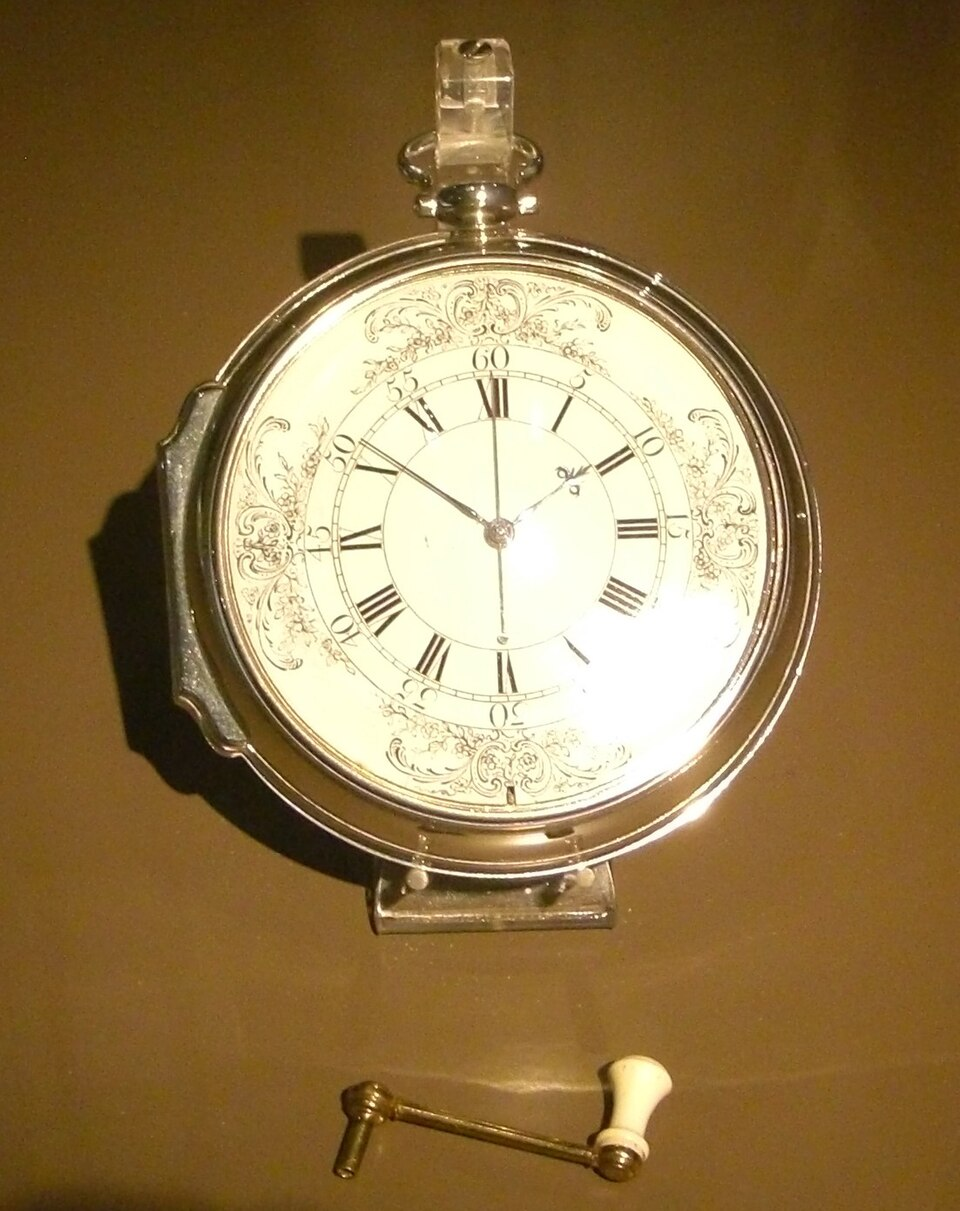
\includegraphics[width=\linewidth]{images/book1/g6-harrison-h4.jpg}\\[2pt]
{\footnotesize H4 karya Harrison, National Maritime Museum, Greenwich. (Foto:
Colonel Warden, CC BY-SA 3.0, melalui Wikimedia Commons.)}
% ledger: commons:harrison-h4
\end{minipage}
\end{history}

\section{Latihan}

\begin{exercise}[$\star$]\label{exo:g6:latitude-longitude:1}
Salin dan lengkapi: ``\omterm{def:g6:latitude-longitude:latitude}{Lintang} diukur dari \ldots{} dan bernilai dari
$0^\circ$ sampai \ldots; \omterm{def:g6:latitude-longitude:longitude}{bujur} diukur dari \omterm{def:g6:latitude-longitude:longitude}{meridian} \ldots{} dan bernilai
dari $0^\circ$ sampai \ldots''
\end{exercise}

\begin{exercise}[$\star$]\label{exo:g6:latitude-longitude:2}
Berapakah \omterm{def:g6:latitude-longitude:latitude}{lintang} \omterm{def:g3:continents-and-oceans:poles}{Kutub Utara}? \omterm{def:g6:latitude-longitude:latitude}{Lintang} \omterm{def:g3:continents-and-oceans:poles}{Kutub Selatan}? \omterm{def:g6:latitude-longitude:latitude}{Lintang} sebuah kota di
\omterm{def:g3:continents-and-oceans:equator}{khatulistiwa}?
\end{exercise}

\begin{exercise}[$\star$]\label{exo:g6:latitude-longitude:3}
Dengan memakai \omterm{def:g2:drawing-to-map:map}{peta} tiga belas kota, sebutkan di \omterm{def:g3:continents-and-oceans:equator}{belahan bumi} mana, utara
atau selatan, dan di sisi mana dari \omterm{def:g6:latitude-longitude:longitude}{meridian utama}, timur atau barat,
setiap kota berikut terletak: Sydney, New York, Kairo, Rio de Janeiro.
\end{exercise}

\begin{exercise}[$\star$]\label{exo:g6:latitude-longitude:4}
Benar atau salah? Perbaiki kalimat yang salah.
(a) Semua \omterm{def:g6:latitude-longitude:longitude}{meridian} bertemu di \omterm{def:g3:continents-and-oceans:poles}{kutub}.
(b) Semua \omterm{def:g6:latitude-longitude:latitude}{paralel} sama panjang.
(c) \omterm{def:g3:continents-and-oceans:equator}{Khatulistiwa} adalah sebuah \omterm{def:g6:latitude-longitude:latitude}{paralel}.
(d) \omterm{def:g6:latitude-longitude:longitude}{Meridian utama} melalui Paris.
\end{exercise}

\begin{exercise}[$\star\star$]\label{exo:g6:latitude-longitude:5}
Dengan memakai \omterm{def:g2:drawing-to-map:map}{peta} tiga belas kota, kota manakah yang terletak pada
kira-kira $30^\circ$\,LU, $31^\circ$\,BT? Kota manakah yang terletak pada
kira-kira $41^\circ$\,LU, $74^\circ$\,BB? Berikan koordinat perkiraan Tokyo.
% ledger: data:b1-ne-places (cities.py main table)
\end{exercise}

\begin{exercise}[$\star\star$]\label{exo:g6:latitude-longitude:6}
Kota~A terletak pada \omterm{def:g6:latitude-longitude:longitude}{bujur} $0^\circ$ dan kota~B pada \omterm{def:g6:latitude-longitude:longitude}{bujur} $45^\circ$\,BT.
Berapa jam selisih tengah hari kedua kota itu? Di kota manakah tengah hari
terjadi lebih dahulu?
\end{exercise}

\begin{exercise}[$\star\star$]\label{exo:g6:latitude-longitude:7}
Mumbai terletak pada kira-kira $73^\circ$\,BT. Tentukan \omterm{def:g6:latitude-longitude:time-zone}{zona waktu} idealnya.
Ketika di Greenwich pukul 12.00 siang, pukul berapakah di Mumbai, menurut
zona ideal?
% ledger: data:b1-ne-places (cities.py: 72.88 E, zone +5)
\end{exercise}

\begin{exercise}[$\star\star$]\label{exo:g6:latitude-longitude:8}
Setiap derajat \omterm{def:g6:latitude-longitude:latitude}{lintang} panjangnya kira-kira \qty{111}{km}. Seberapa jauh dari
\omterm{def:g3:continents-and-oceans:equator}{khatulistiwa} letak sebuah kota pada $30^\circ$\,LU, diukur sepanjang
\omterm{def:g6:latitude-longitude:longitude}{meridiannya}? Seberapa jauh \omterm{def:g3:continents-and-oceans:poles}{Kutub Utara} dari \omterm{def:g3:continents-and-oceans:equator}{khatulistiwa}?
% ledger: rmg:latitude-def
\end{exercise}

\begin{exercise}[$\star\star$]\label{exo:g6:latitude-longitude:9}
New York berada di zona $-5$ dan Tokyo di zona $+9$. Berapa jam selisih jam
di kedua kota itu? Ketika di New York pukul 08.00 hari Senin, pukul berapa
dan hari apakah di Tokyo?
% ledger: data:b1-ne-places (cities.py: zones -5 and +9)
\end{exercise}

\begin{exercise}[$\star\star$]\label{exo:g6:latitude-longitude:10}
Lena berkata: ``Matahari terbit di timur, jadi kota-kota di timur melihat
Matahari terbit lebih dahulu daripada kota-kota di barat.'' Apakah ia benar?
Jelaskan dengan perputaran Bumi.
\end{exercise}

\begin{exercise}[$\star\star\star$]\label{exo:g6:latitude-longitude:11}
Jam sebuah kapal bertambah cepat 3~detik sehari (jam itu berjalan terlalu
cepat). (a) Berapa detik jam itu terlalu cepat setelah pelayaran selama
42~hari? (b) Bumi berputar satu derajat dalam 4~menit, yaitu 240~detik.
Berapa kesalahan, dalam derajat \omterm{def:g6:latitude-longitude:longitude}{bujur}, yang ditimbulkan oleh kesalahan jam
itu? (c) Di \omterm{def:g3:continents-and-oceans:equator}{khatulistiwa}, satu derajat \omterm{def:g6:latitude-longitude:longitude}{bujur} panjangnya kira-kira
\qty{111}{km}. Kira-kira berapa kilometer kesalahan sang navigator, di
\omterm{def:g3:continents-and-oceans:equator}{khatulistiwa}?
% ledger: rmg:longitude-act-1714, rmg:15deg-per-hour, rmg:latitude-def
\end{exercise}

\begin{exercise}[$\star\star\star$]\label{exo:g6:latitude-longitude:12}
Sebuah pesawat berangkat dari Tokyo (zona $+9$) pada pukul 18.00 hari Senin
dan terbang ke timur melintasi Pasifik menuju Los Angeles (zona $-8$).
Penerbangan itu berlangsung 10~jam. (a) Pukul berapakah di Greenwich ketika
pesawat berangkat? (b) Pukul berapakah di Greenwich ketika pesawat mendarat?
(c) Pukul berapa waktu setempat dan hari apakah di Los Angeles ketika
pesawat mendarat? Mengapa para pelancong mengatakan bahwa pada penerbangan
ini ``kamu mendarat sebelum kamu lepas landas''?
\end{exercise}

\section{Soal: Panggilan Video Keliling Dunia}

\begin{problem}[{Soal akhir pekan --- lima sahabat, empat zona waktu, dan satu
garis batas tanggal: pukul berapa di Auckland ketika panggilan dimulai?}]
\label{pb:g6:latitude-longitude:1}
% ledger: data:b1-ne-places, rmg:15deg-per-hour, planet:Earth.day (cities.py, time_zones.py; test_cities_zones_used_in_the_problem)
Lena tinggal di London. Ia ingin mengadakan panggilan video dengan empat
temannya yang ia kenal saat berlibur: Ana di Rio de Janeiro, Kenji di Tokyo,
Mia di Auckland, dan Sam di Los Angeles. Dalam soal ini, kita memakai \omterm{def:g6:latitude-longitude:time-zone}{zona
waktu} ideal.

\begin{center}
\small
\begin{tabular}{lll}
\hline
teman & kota & koordinat\\
\hline
Lena & London & $52^\circ$\,LU, $0^\circ$\\
Ana & Rio de Janeiro & $23^\circ$\,LS, $43^\circ$\,BB\\
Kenji & Tokyo & $36^\circ$\,LU, $140^\circ$\,BT\\
Mia & Auckland & $37^\circ$\,LS, $175^\circ$\,BT\\
Sam & Los Angeles & $34^\circ$\,LU, $118^\circ$\,BB\\
\hline
\end{tabular}
\end{center}

\medskip
\noindent\textbf{Bagian I --- Tempat tinggal para sahabat.}
\begin{enumerate}
  \item Teman-teman mana yang tinggal di \omterm{def:g3:continents-and-oceans:equator}{belahan bumi selatan}?
  \item Teman-teman mana yang tinggal di barat \omterm{def:g6:latitude-longitude:longitude}{meridian utama}?
  \item Teman mana yang tinggal paling jauh dari \omterm{def:g3:continents-and-oceans:equator}{khatulistiwa}?
  \item Teman mana yang tinggal paling dekat dengan \omterm{def:g6:latitude-longitude:longitude}{meridian} $180^\circ$?
        Berapa derajat \omterm{def:g6:latitude-longitude:longitude}{bujur} jaraknya dari \omterm{def:g6:latitude-longitude:longitude}{meridian} itu?
\end{enumerate}

\medskip
\noindent\textbf{Bagian II --- Pukul berapa sekarang?}
\begin{enumerate}[resume]
  \item Berapa derajat Bumi berputar dalam satu jam?
  \item Tentukan \omterm{def:g6:latitude-longitude:time-zone}{zona waktu} ideal kota setiap teman.
  \item Lena mengusulkan agar panggilan dimulai pada hari Jumat pukul 20.00,
        waktu London. Pukul berapa dan hari apakah saat itu di Rio de
        Janeiro? Di Tokyo?
  \item Kenji menjawab bahwa ia pasti sedang tidur. Jelaskan mengapa di
        Tokyo sudah hari Sabtu.
\end{enumerate}

\medskip
\noindent\textbf{Bagian III --- Menyeberangi garis batas tanggal.}
\begin{enumerate}[resume]
  \item Pukul berapa dan hari apakah di Los Angeles ketika panggilan
        dimulai?
  \item Berapa jam jam di Auckland lebih dahulu daripada jam di Los Angeles?
  \item Ketika berlayar ke timur dari Auckland menuju Los Angeles, sebuah
        kapal menyeberangi \omterm{def:g6:latitude-longitude:date-line}{garis batas tanggal}. Apakah kapal itu maju ke hari
        berikutnya atau mundur ke hari sebelumnya?
  \item Pukul berapa waktu setempat, dan hari apakah, di Auckland ketika
        panggilan dimulai?
\end{enumerate}
\end{problem}
